%% This is an example first chapter.  You should put chapter/appendix that you
%% write into a separate file, and add a line \include{yourfilename} to
%% main.tex, where `yourfilename.tex' is the name of the chapter/appendix file.
%% You can process specific files by typing their names in at the 
%% \files=
%% prompt when you run the file main.tex through LaTeX.
\chapter{Introduction}
\begin{quotation}

\textit{``Some people write poetry in the language we speak. Perhaps better poetry will be written in the language of digital computers of the future than has ever been written in English."}
-J.C.R Licklider
\end{quotation}


Computation is a driving force in our world. The power and ubiquity of  modern computer systems have made the skill of computer programming relevant to a wide range of human studies and disciplines. Commonly, programming is viewed as an essential component of science, engineering and business. Despite this view, computation is also a powerful tool for creative disciplines. When applied to the arts, programing offers different paradigms for creation and new methods of problem solving. My personal interest in this respect lies in computational design: the use of programing to generate visual form. Frequently used to create screen-based work, computational design is also applicable to the design of physical objects. The advent of digital-fabrication technology allows for a transition from digital forms produced by computation to physical artifacts that live in the world. The joint use of computational design and digital fabrication is becoming an integral component  of professional art and design, both as a method of prototyping and as a means for producing finished work. Although these technologies primarily serve professionals, the combination of computational design and digital fabrication also provides the opportunity for amateur creative expression. The growing diversity in programing environments, combined with the emergence of the personal fabrication movement suggest new ways to support non-professionals in a combined practice of computation, design and construction. In addition, many forms of digital fabrication are compatible with traditional art and craft techniques. The combination of computational design and digital fabrication provides a way of making programing relevant to people with an interest in craft.  The development of accessible computational-design and digital-fabrication tools therefore presents new opportunities for broadening participation in programming, expanding the ways in which people create, and changing the role programing can play in people's lives.

 \begin{center}
 \begin{figure}[h!]
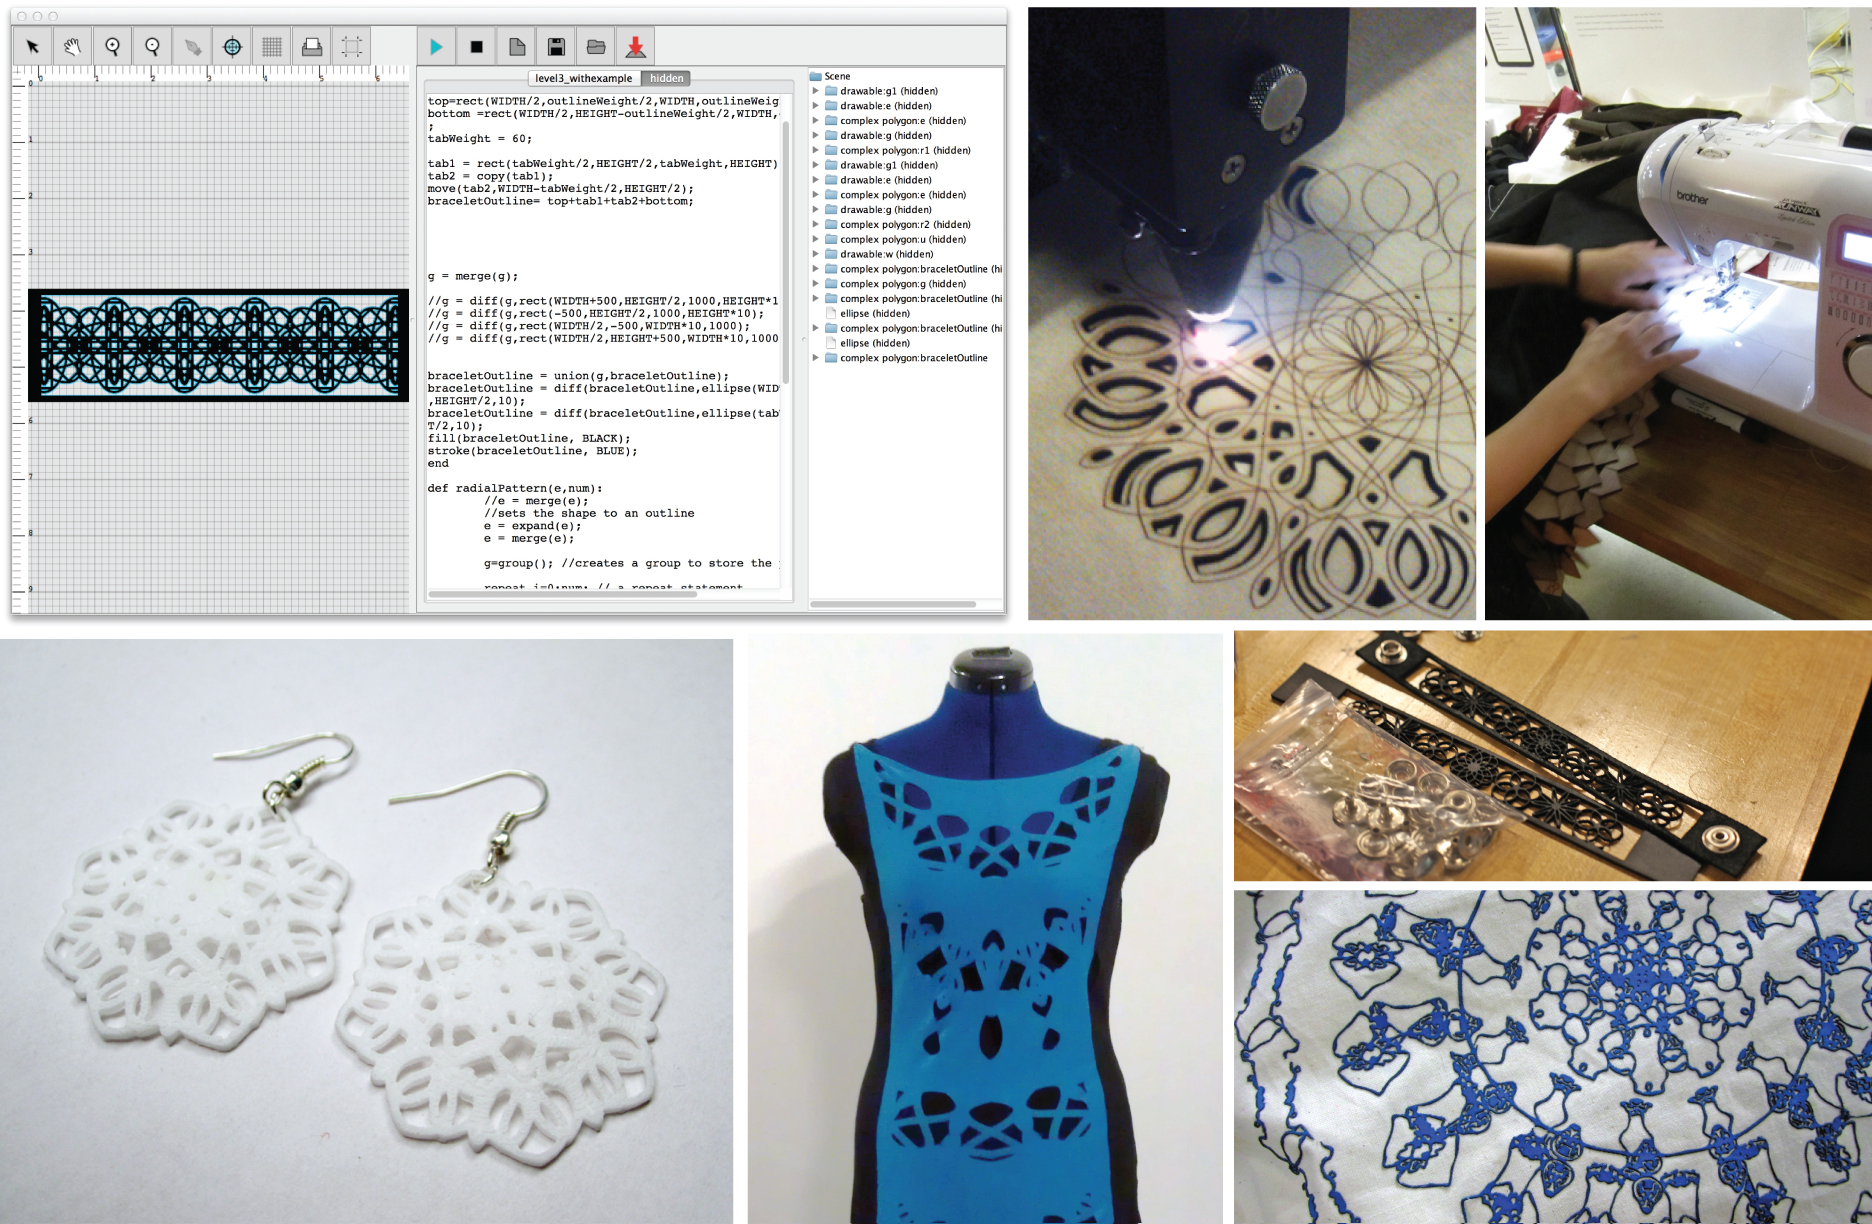
\includegraphics[width=\columnwidth]{images/intro_pic.jpg}
\caption{Algorithmic craft practices, tools and artifacts. }
\label{fig:intro}
\end{figure}
\end{center}

In this thesis, I examine methods that facilitate participation in the intersection of computational design, digital fabrication and traditional arts and crafts for the production of functional and decorative physical artifacts. I use the term algorithmic craft as a way of describing these collective practices. My primary aim is to support people without formal education or experience in computer science in the practice of algorithmic craft, although I also seek to develop methods that are accessible to individuals without formal training in art and design. My goal is to work with people in ways that emphasize pleasure, recreation and non-professional utility in the service of personal expression. 

My study of this space is motivated by the practical and theoretical questions that arise when bridging the spaces between textual programming language, visual design, and machine and hand-based physical construction. What are the important design principles to consider when creating  programming environments for physical design? How do we compellingly link textual code with visual designs, and what are the appropriate intersection points between textual manipulation and visual manipulation? What support is required to help people move back and forth from programming to building real objects in a way that is comfortable, expressive and pleasurable? How can we remove the technical challenges in translating code into an object that can be successfully fabricated, while still supporting a wide variety of design styles, aesthetics and approaches? Finally, how can we interlink the often disparate processes of physical prototyping with digital design and programming in a way that creatively reinforces both physical and virtual modes of working?

In order to address these questions,  I developed three different software tools to support practitioners in this domain. Codeable Objects is a programing library that helps people design and fabricate laser-cut lamps. Soft Objects is an extension of Codeable Objects that allows people to use programing to create forms and patterns for fashion and garment design. DressCode is a combined graphic-design and programing environment with a custom programing language, developed to support open-ended computational design for digital fabrication. Each of these tools were evaluated in workshops where people used them in combination with digital fabrication machines to produce physical artifacts. Through the workshops, I examined several different approaches for introducing novices to computational design. In addition, I evaluated how a variety of crafting techniques could be combined with Computer Aided Design (CAD). The lessons learned in developing and testing Codeable Objects and Soft Objects were used to inform the development of DressCode. This thesis presents the evolution of these three tools, and describes the rationale behind their design. I conclude with a discussion of some of the unique affordances of algorithmic craft, and the possibilities it offers for creative expression in the future.  \todo{this may change.. be sure to check}